

\documentclass[12pt,a4paper]{article}
\newcommand\persiangloss[2]{#1\dotfill\lr{#2}\\}
\usepackage{graphicx}
\usepackage{xcolor}
\usepackage{listings}
\usepackage{indentfirst}
\usepackage{float}
\usepackage[pagebackref=false,colorlinks,linkcolor=blue,citecolor=magenta]{hyperref}
\usepackage{xepersian}
\settextfont{XB Niloofar}
\definecolor{vgreen}{RGB}{104,180,104}
\definecolor{vblue}{RGB}{49,49,255}
\definecolor{vorange}{RGB}{255,143,102}

\lstdefinestyle{verilog-style}
{
	language=Verilog,
	basicstyle=\small\ttfamily,
	keywordstyle=\color{vblue},
	identifierstyle=\color{black},
	commentstyle=\color{vgreen},
	numbers=left,
	numberstyle=\tiny\color{black},
	numbersep=10pt,
	tabsize=8,
	moredelim=*[s][\colorIndex]{[}{]},
	literate=*{:}{:}1
} 



\begin{document}
	\thispagestyle{empty}
	\vspace*{0mm}
	\centerline{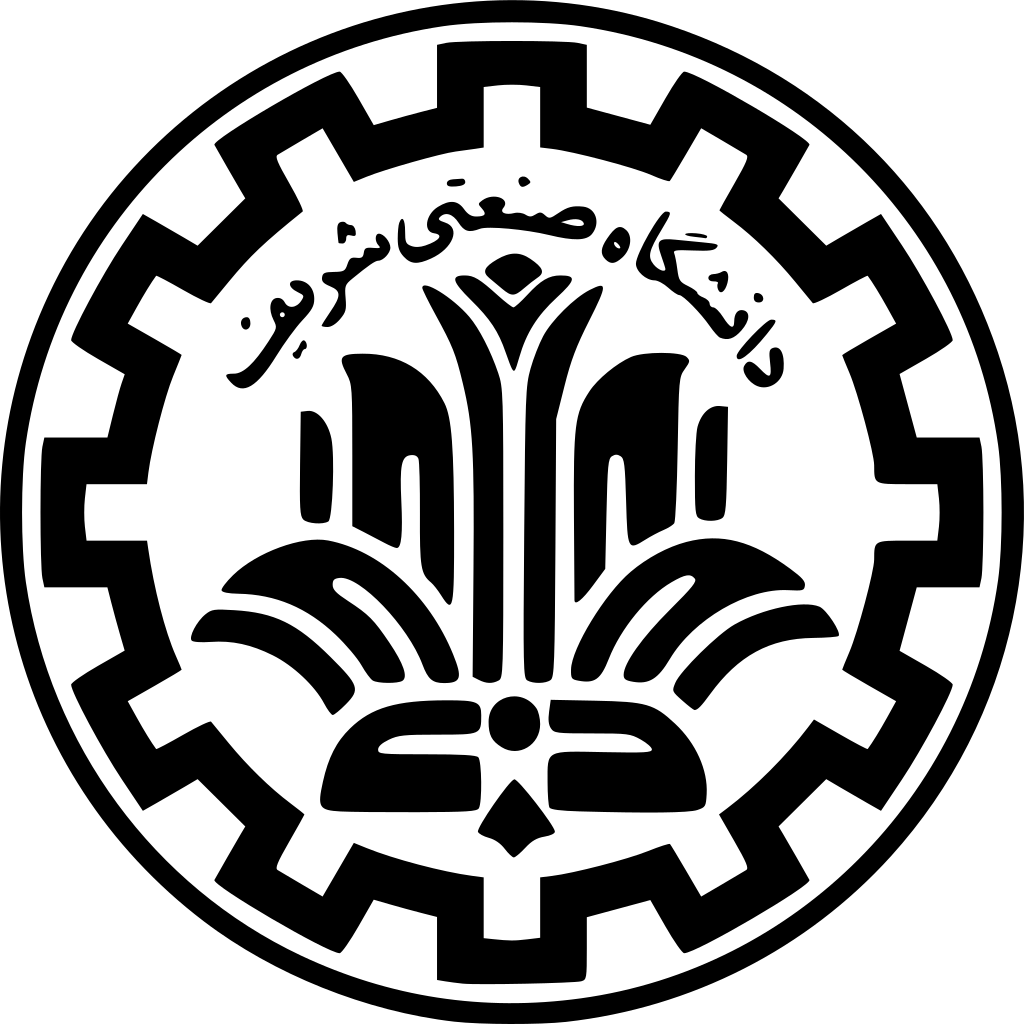
\includegraphics[height=4cm]{logo.png}}
	\vspace*{5mm}
	\begin{center}
		{\Huge
لوستر هوشمند - گزارش دوم
}
\\[1cm]
آزمایشگاه سخت‌افزار
\\[1cm]
دانشکده مهندسی کامپیوتر
\\[4cm]
{\large
محمدرضا عبدی ۹۷۱۱۰۲۸۵

حمیدرضا کامکاری ۹۷۱۱۰۱۷۷

یگانه قره‌داغی 97106216
}
	\\[5cm]
	فروردین ۱۴۰۱
	\end{center}
\newpage

\section*{گزارش دوم}

در این آزمایش ماژول 
\lr{BH1750}
برای تشخیص نور را بورد آردویینو طبق شکل
\ref{fig:schema}
 وصل کردیم. همانطور که می‌بینید پورت‌های
 \lr{SCL}
 و
 \lr{SDA}
 به پورت مربوطه با همان اسم در آردویینو متصل شده‌اند. 
 \lr{VCC}
 را به ۵ ولت و 
 \lr{ADO}
 و
 \lr{GND}
 را به زمین متصل کردیم.
 \begin{figure}[H]
 	\centering
 	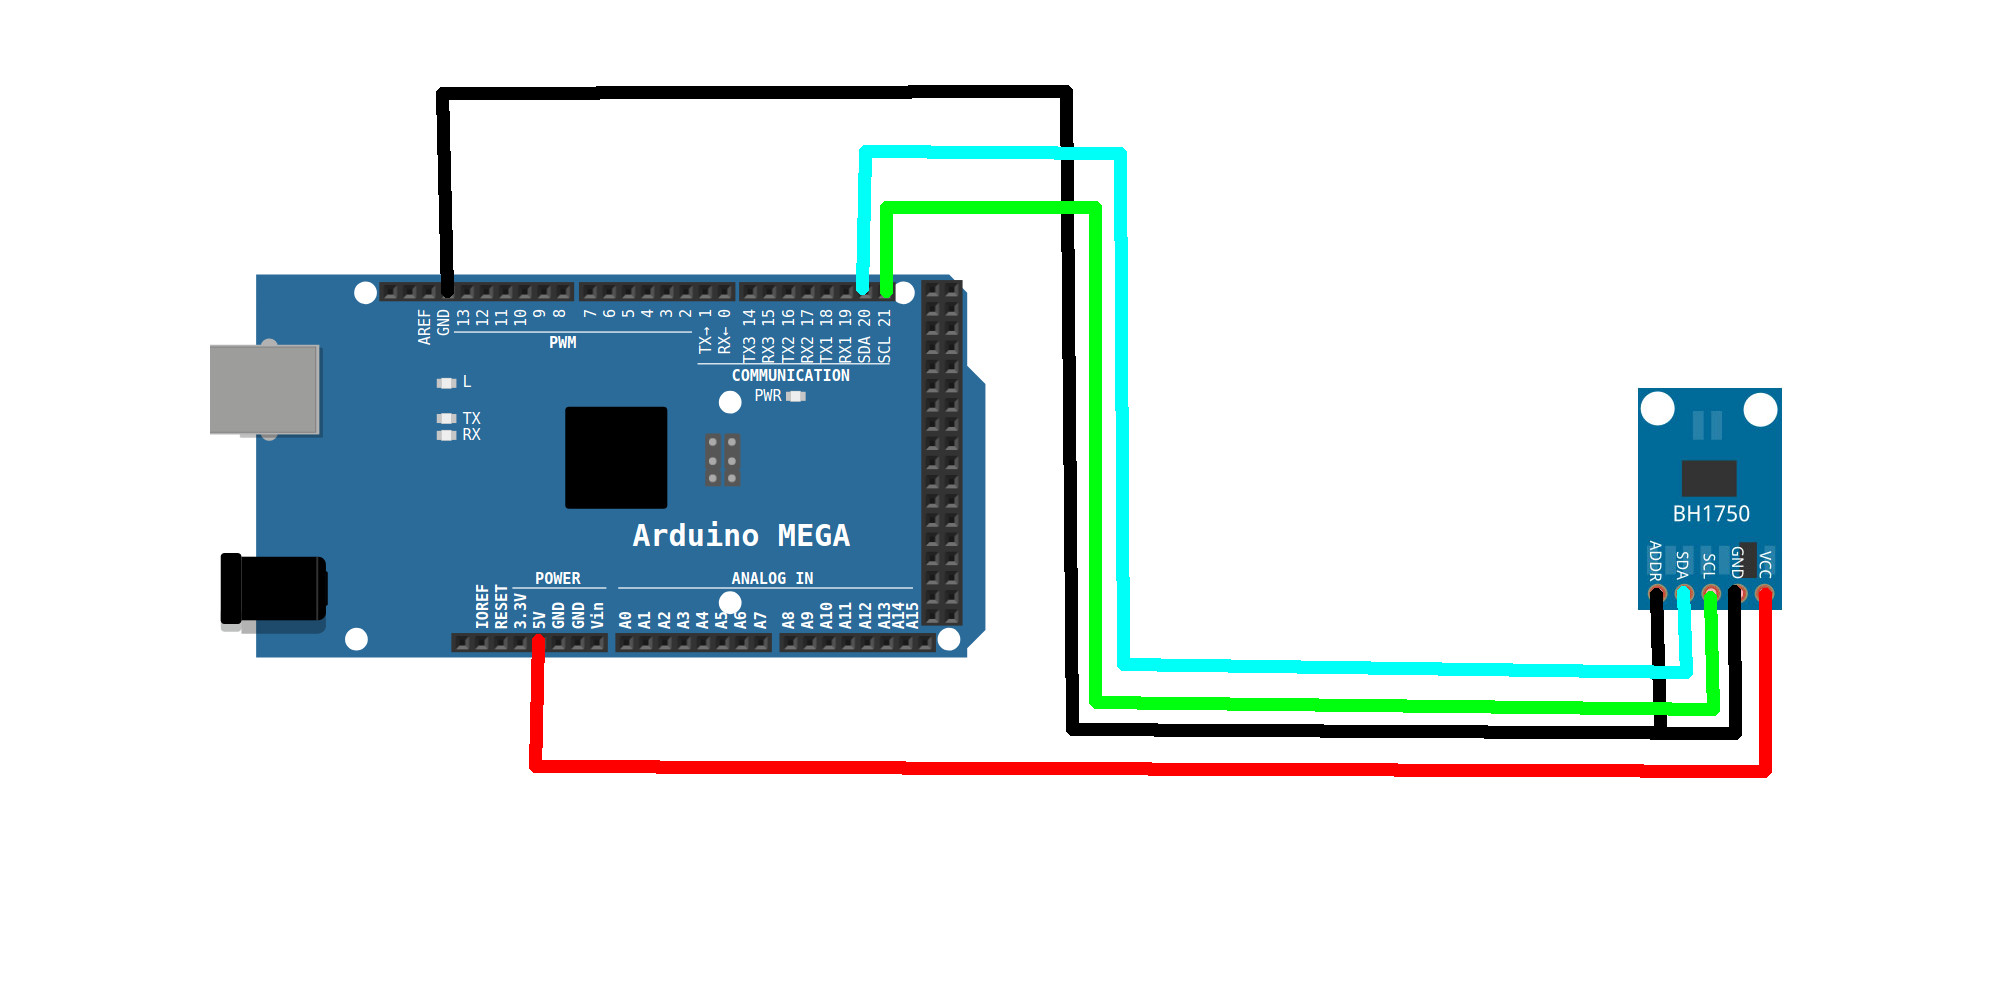
\includegraphics[scale=0.3]{figs/schema.jpg}
 	\caption{
 		شماتیک مدار تشخیص نور.
 	}
 	\label{fig:schema}
 \end{figure}
 
 

هدف از این بخش از کار آشنایی با ساز و کار این ماژول بود و با استفاده از فرمولی ساده ورودی به‌دست آمده از سنسور را با فرمولی تبدیل به 
\lr{Brightness}
ای کردیم که از طریق 
\lr{PWM}
قابل کنترل است. مقدار ورودی سنسور را می‌توان با عددی ممیز شناور در بازه $0$ تا 
$2^16$
مدل کرد. اما به علت کاربرد ما که نور محیطی است، این مقدار خروجی با استفاده از آزمایش مقداری بین $0$ و 
$500$
به دست آمد. پس از 
\lr{scale}
کردن این مقدار بین صفر و یک و استفاده از فرمول
$$inv(lux) = (1 - lux)^4$$
مقدار روشنایی خروجی را بین صفر و یک به دست آوردیم که پس از ضرب شدن در 
$255$
به ما عدد روشنایی 
\lr{LED}
ها را می‌دهد. توجه کنید قدرت تشخیص نور انسان به صورت خطی نیست و قدرت تفکیک در بین روشنایی‌های پایینتر بیشتر است. لذا تابعی شبه‌نمایی برای تبدیل معکوس مناسب است که شکل نمودار 
$x^4$
چنین خواسته‌ای را برطرف می‌کند. از طرفی از 
$(1 - x)^4$
استفاده کردیم که خروجی سنسور با میزان نور رابطه عکس داشته باشد و نور در محیط تاریک بیشتر و در محیط روشن کمتر شود. شکل نمودار در شکل
\ref{fig:plot}
موجود است.
\begin{figure}[H]
	\centering
	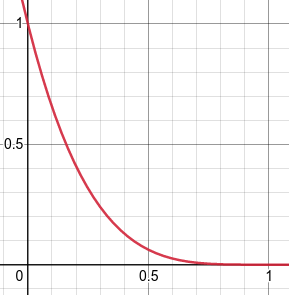
\includegraphics[scale=0.6]{figs/inversion-formula-plot.png}
	\caption{
		شکل نمودار مورد استفاده برای معکوس کردن خروجی سنسور برای به‌دست آوردن خروجی 
		\lr{LED}.
	}
	\label{fig:plot}
\end{figure}

ویدیو‌ای از تست کردن این مدار به اسم
\lr{video-week2.MOV}
در ریپوزیتوری پروژه ذخیره شده‌است. برای چک کردن صحت، سنسور را در وضعیتی که روی میز باشد قرار دادیم که تاریکی مطلق است، در جلوی نور لامپ قرار دادیم و نهایتا با استفاده از چراغ قوه گوشی نوری با شدت بسیار زیاد تابیدیم. نتایج به ترتیب در شکل‌های \ref{fig:dark}، \ref{fig:normal} و \ref{fig:torch} موجود است و همانطور که ی‌بینید به ترتیب کاملا روشن، نیمه‌روشن و کاملا خاموش است.


\begin{figure}[H]
	\centering
	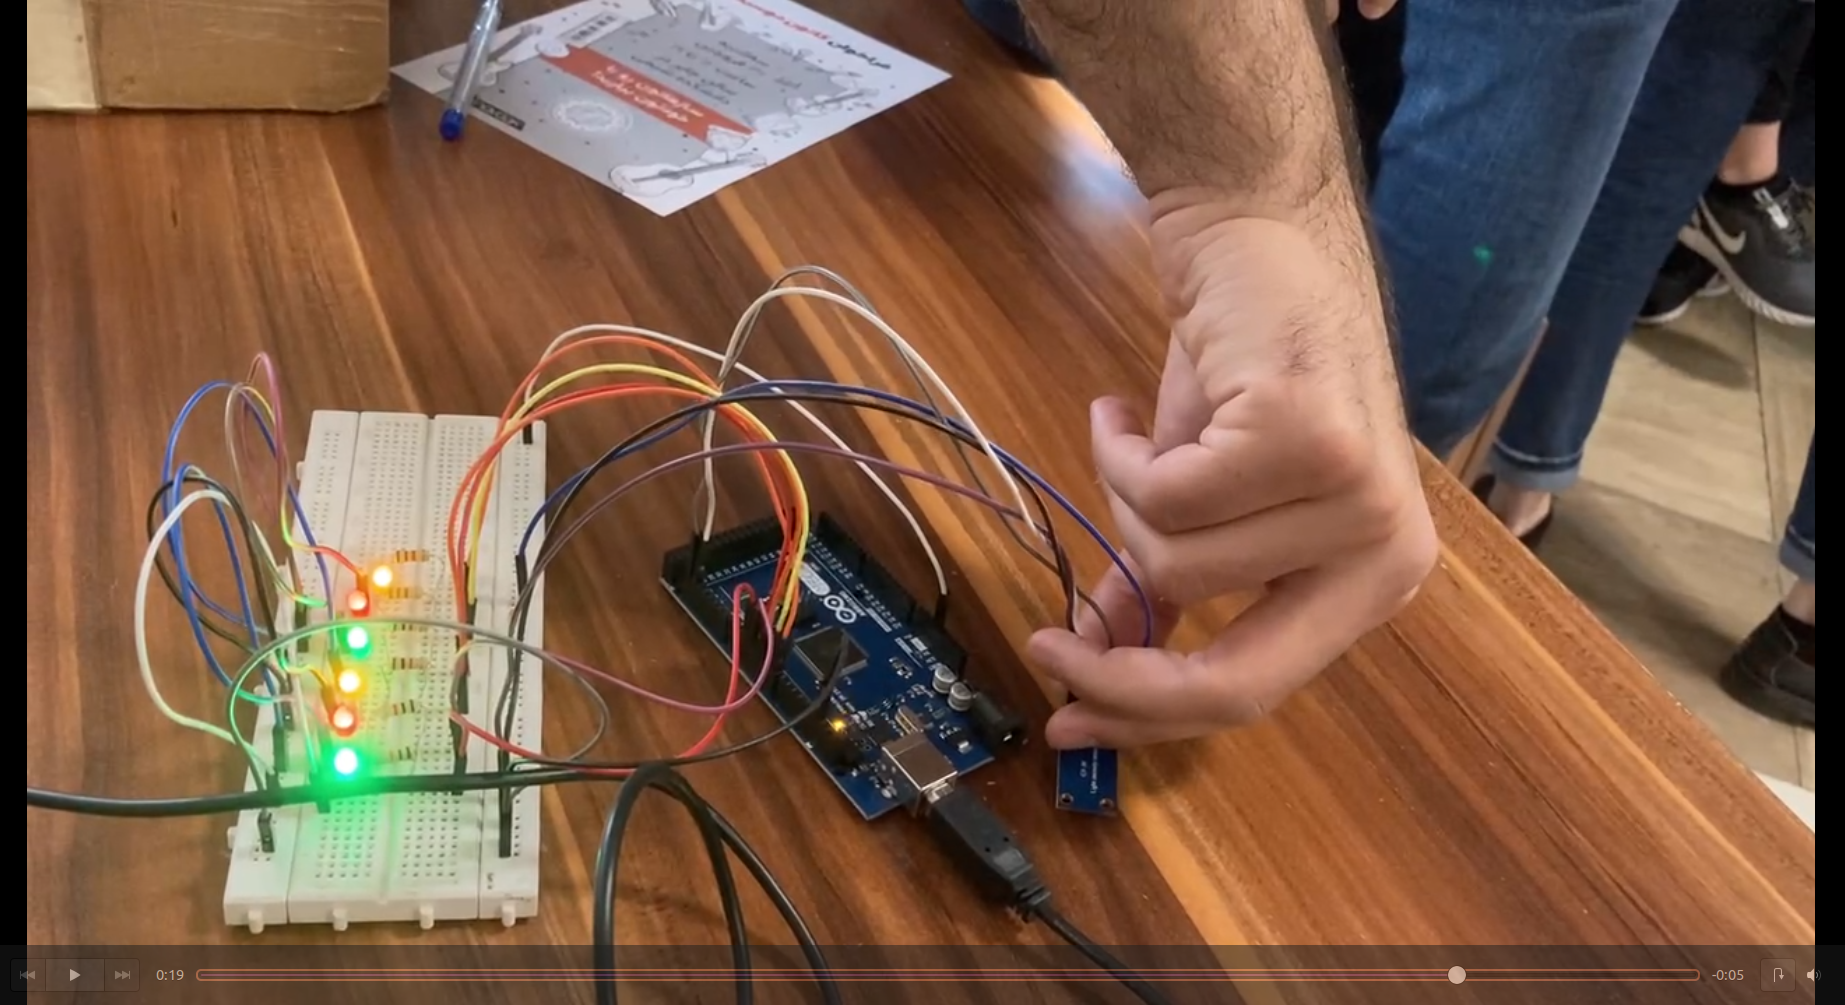
\includegraphics[scale=0.2]{figs/dark-light.png}
	\caption{
		میزان روشنایی
		\lr{LED}
		ها هنگامی که سنسور روی میز و در تاریکی مطلق قرار دارد که همانطور که می‌بینید چراغ‌ها در روشن ترین حالت خود هستند.}
	\label{fig:dark}
\end{figure}

\begin{figure}[H]
	\centering
	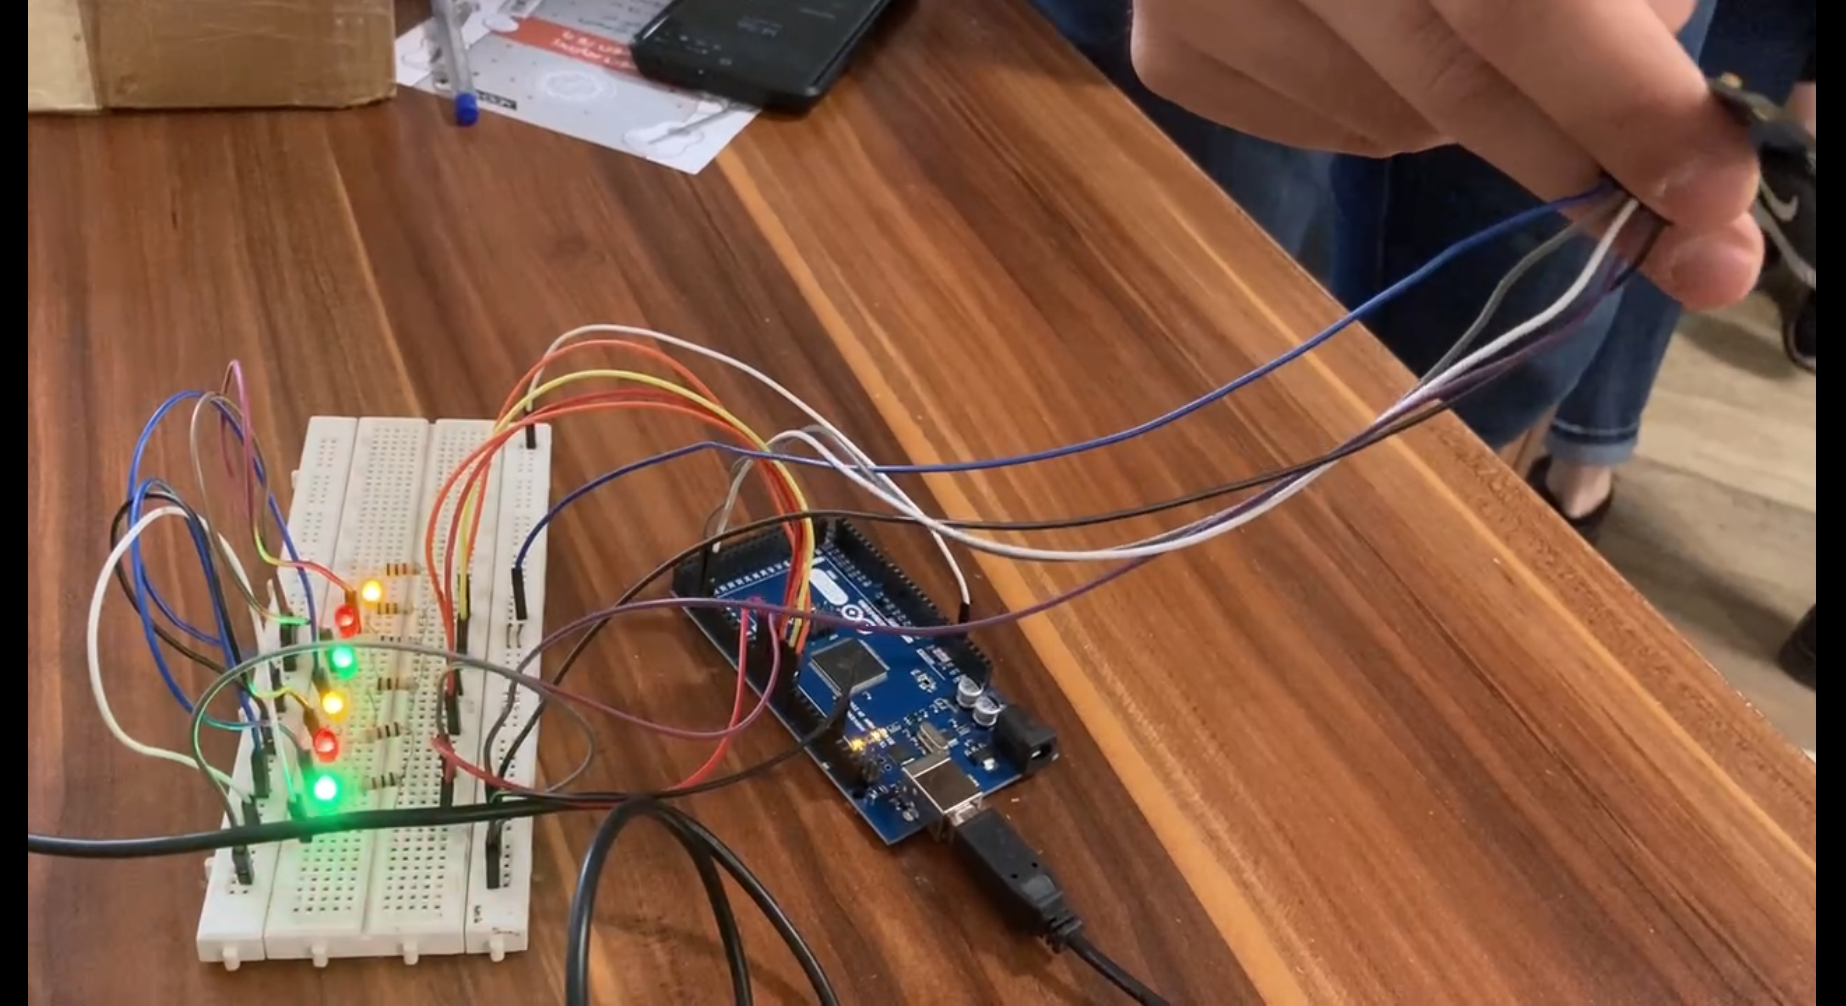
\includegraphics[scale=0.2]{figs/normal-light.png}
	\caption{میزان روشنایی 
\lr{LED}
ها هنگامی که سنسور در برابر نور لامپ قرار دارد.	
}
	\label{fig:normal}
\end{figure}




\begin{figure}[H]
	\centering
	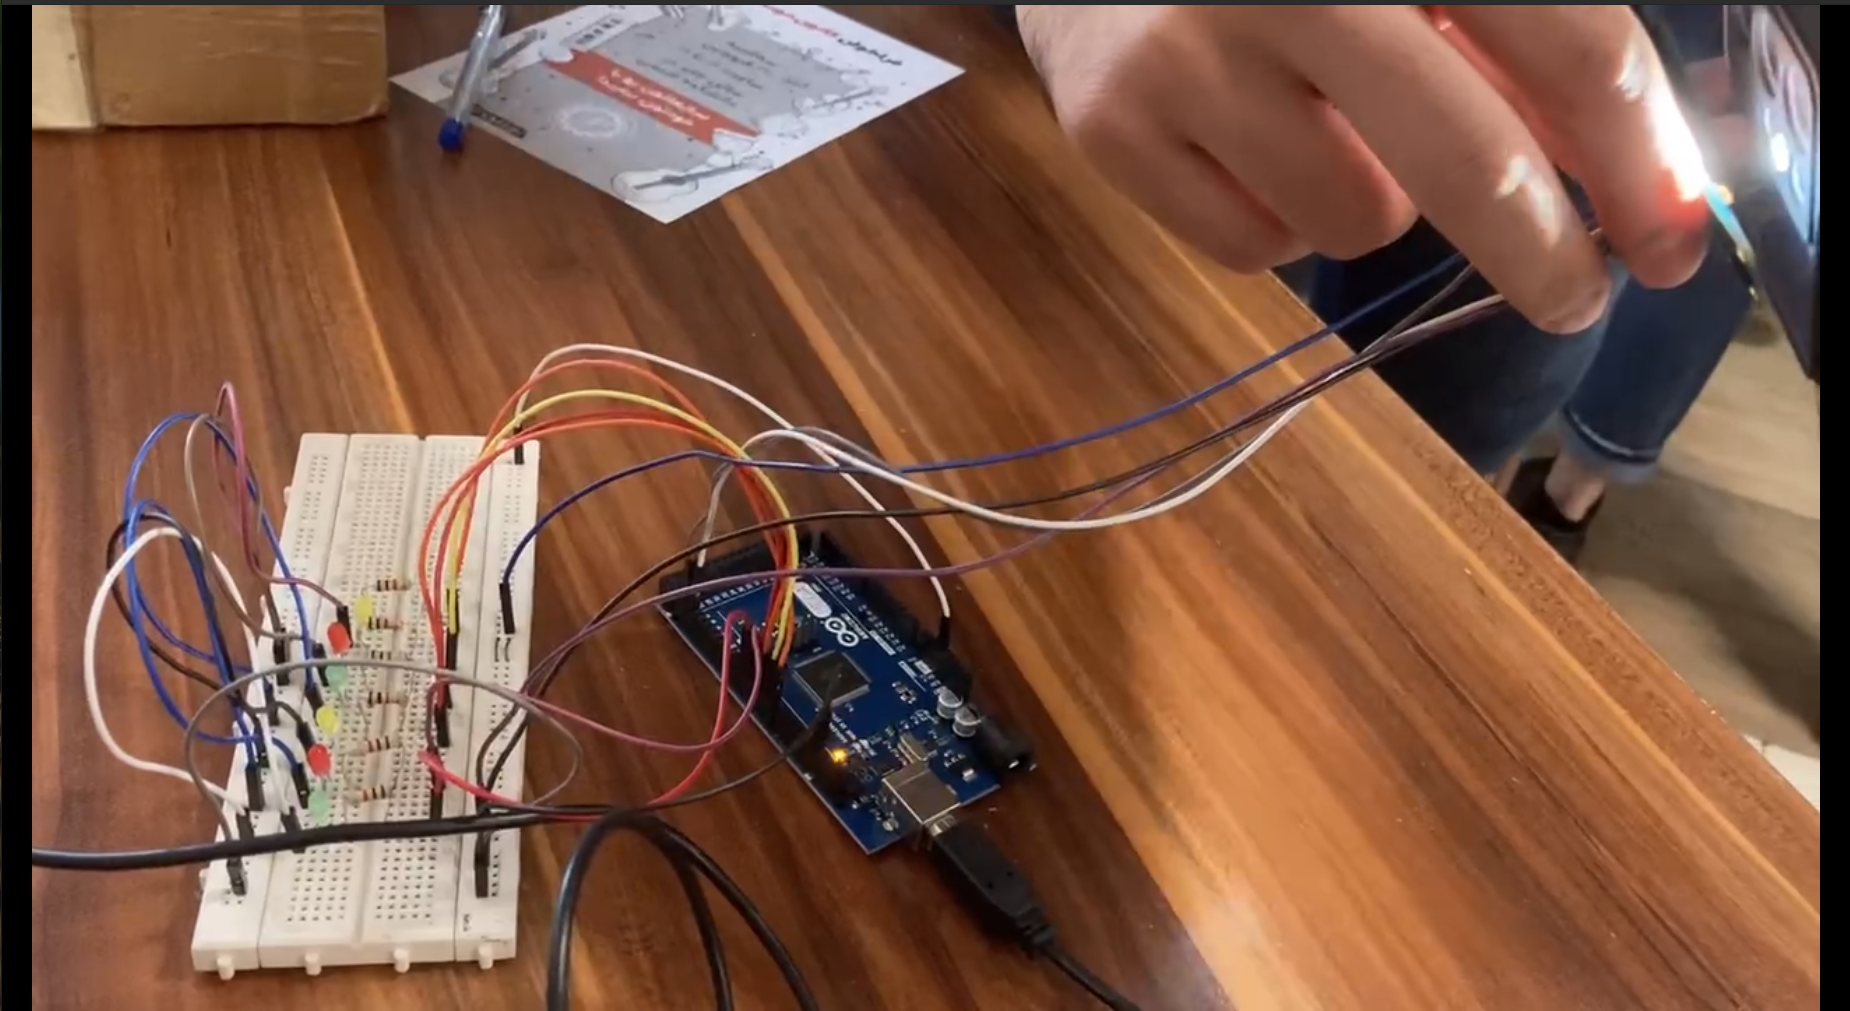
\includegraphics[scale=0.2]{figs/extreme-light.png}
	\caption{
		میزان روشنایی 
		\lr{LED}
		ها هنگامی که سنسور جلوی نور شدید چراغ‌ قوه‌ی گوشی قرار دارد، همانطور که می‌بینید در این حالت 
		\lr{LED}
		ها خاموش می‌شوند.	
	}
	\label{fig:torch}
\end{figure}

در ادامه می‌توانید کد مربوط به این کار را ببینید:
\begin{latin}
	\lstinputlisting[style={verilog-style}]{src/sensor-LED.ino}
\end{latin}

\end{document}